\chapter{Reconstrucción e identificación de objetos físicos}
\label{ch:objects}
\epigraph{\emph{``Experiment is the sole judge of scientific truth.”}}{Richard Feynman}


Las partículas producidas en cada colisión y los productos de sus decaimientos interactúan con el detector de una manera particular según su naturaleza. La información recogida por todos los subdetectores de \ac{ATLAS} permite reconstruir e identificar los objetos físicos presentes en cada evento aceptado por el sistema de trigger (selección \textit{online}). En este capítulo se describen los algoritmos de reconstrucción e identificación \textit{offline} que se lleva a cabo una vez que los eventos han sido aceptados por el trigger y almacenados. La reconstrucción se realiza evento por evento utilizando los mismos algoritmos para los eventos recolectados por el detector \ac{ATLAS} y para los eventos simulados con \acf{MC}. A continuación se da un breve resumen de la reconstrucción offline y la identificación de los objetos utilizados en esta tesis.




\section{Reconstrucción de trazas y vértices}

En un evento con alto pileup puede haber del orden de 1000 partículas cargadas pasando por el detector \ac{ATLAS}. La información del \ac{ID} (\Sect{\ref{subsec:atlas:atlas:id}}) se utiliza para reconstruir las trayectorias de las partículas cargadas, denominadas trazas (\textit{tracks}).
Dado que el \ac{ID} es el detector más cercano al haz y está compuesto por material mínimamente ionizante con una granularidad elevada, este detector desempeña el papel principal en la reconstrucción de trazas. Estas permiten calcular el momento y la trayectoria de las partículas cargadas dejando una señal en las diferentes capas del \ac{ID}. Además, como el campo solenoidal dentro del \ac{ID} es homogéneo, la trayectoria resultante es circular en el plano \(xy\). Cinco parámetros mostrados en la \Fig{\ref{fig:objects:track_vtx:track_parameters}} definen las trazas de las partículas cargadas:
\begin{itemize}
    \item \(q/\pt\): la relación entre la carga y el momento transverso que define la curvatura.
    \item \(d_0\): la distancia de máxima aproximación al vértice primario en el plano-\(xy\) que define el parámetro de impacto transversal.
    \item \(z_0\): el parámetro de impacto longitudinal a lo largo del eje \(z\).
    \item \(\phi_0\): el ángulo azimutal.
    \item \(\theta_0\): el ángulo polar de la dirección de la partícula en el punto más cercano de aproximación~\cite{ATLAS-Tracks-Performance-Run2}.
\end{itemize}

\begin{figure}[ht!]
    \centering
    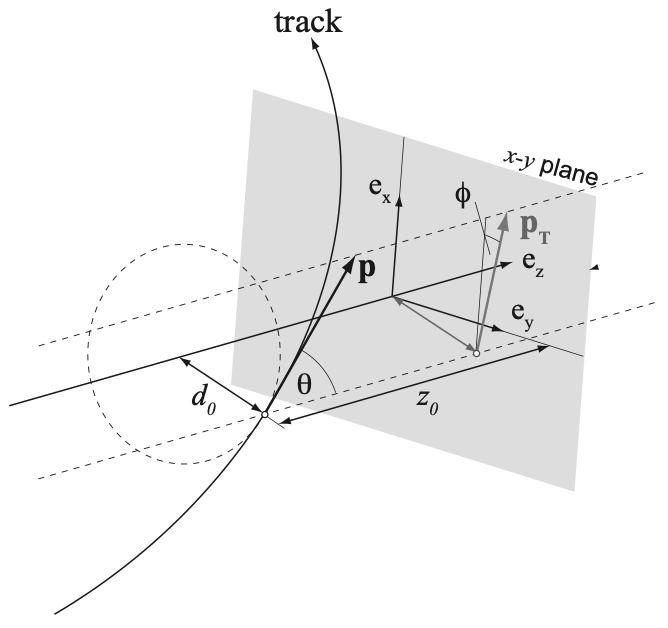
\includegraphics[width=0.6\linewidth]{3_experiment/object_reconstruction/tracking_coordinates.png}
    \caption{Esquema de los parámetros usados para la reconstrucción de trazas~\cite{ATLAS-Tracking-2007}.}
    \label{fig:objects:track_vtx:track_parameters}
\end{figure}

La reconstrucción de trazas utilizada durante el Run-2 utiliza dos enfoques complementarios: el enfoque \textit{inside-out} y el \textit{outside-in}~\cite{ATLAS-NEWT}.

El primer paso para la reconstrucción de trazas en el método inside-out es la búsqueda de semillas (\textit{seeds}), en la que se buscan tres hits en el detector de silicio para comenzar la reconstrucción de la traza. A partir de estos tres hits y suponiendo un campo magnético uniforme se obtiene una primera estimación de los parámetros de la traza. A partir de las seeds de la traza, ésta se extrapola a las demás capas del detector de silicio a partir de las cuales se utiliza un filtro combinatorio de Kalman para estimar los parámetros de la traza. En esta fase del proceso puede haber varias trazas candidatas para cada seed. Una vez formada la traza, se aplica un algoritmo de resolución de ambigüedades para reasignar los clusters compartidos a la traza con mejor coincidencia~\cite{ATLAS-NNClustering} y se ajusta la traza candidata final utilizando un método global \chisq. La última parte del método inside-out consiste en extender las trazas hasta el \ac{TRT} incluyendo los hits de este subdetector para mejorar así la resolución del momento.

Para mejorar la eficiencia de las trazas de los decaimientos desplazados del punto de colisión original se utiliza el método \textit{outside-in}. La reconstrucción de la traza comienza a partir de los hits del \ac{TRT} y luego se extiende para incluir los hits del detector de silicio, aplicándose de nuevo un algoritmo para resolver las ambigüedades mitigando así los hits compartidos entre múltiples trazas.

La identificación de los vértices de producción y decaimiento son de vital importancia para la posterior reconstrucción de objetos en \ac{ATLAS}.
Para ello, un algoritmo de reconstrucción de vértices utiliza las trazas encontradas anteriormente~\cite{ATLAS-PVReconstruction,ATLAS-VertexReconstruction}.

En primer lugar, el \ac{PV} se define como el lugar donde se da la interacción entre los dos protones del \ac{LHC}. Los \acp{PV} se reconstruyen en dos etapas: búsqueda de vértices que asocia las trazas reconstruidas a los candidatos a \ac{PV}; y ajuste de vértices, donde las posiciones de los vértices es refinada de forma iterativa. En cada iteración se selecciona un conjunto de trazas y se utiliza una posición semilla (\textit{seed}) para estimar el vértice. Las trazas incompatibles con este vértice son removidas para una futura iteración.
Finalmente, el vértice con el mayor valor \(\sum \pt^2\) para todas las trazas asociadas, que también se denomina vértice de dispersión dura, se asigna como el \ac{PV}.
Hay algunas partículas que decaen rápidamente después de su producción, como los leptones \(\tau\) o los quarks más pesados (\(b\) o \(\cquarks\)). En \ac{ATLAS}, es posible determinar el vértice de decaimiento del quark \(b\). A partir de las trazas restantes originadas por estos decaimientos, es posible identificar vértices secundarios, y todos los vértices reconstruidos restantes se consideran pileup.








\section{Fotones y electrones}

La reconstrucción de electrones y fotones en \ac{ATLAS} hace uso de las deposiciones de energía en el \ac{ECAL}. Como los electrones y los fotones dejan señales similares en este calorímetro, su reconstrucción se realiza simultáneamente distinguiéndolos por la información de las trazas reconstruidas.


\subsection{Reconstrucción}
\label{subsec:objects:egamma:reco}

La reconstrucción de fotones y electrones \textit{offline}~\cite{ATLAS-EGamma-Performance-2015-2017,ATLAS-TopoClusters-Run2} hace uso de clusters dinámicos de tamaño variable, conectados topológicamente entre las celdas del \ac{ECAL} y \ac{HCAL}~\cite{ATLAS-TopoClusters-Run1}, denominados \textit{\topos} que se agrupan además en \textit{superclusters}. 
Durante el Run-1~\cite{ATLAS-EGamma-Performance-Run1, ATLAS-EGamma-CalibrationPerformance-Run1, ATLAS-CalorimeterClustering-2008}, en contraste, los clusters eran de tamaño fijo y si bien tenían una respuesta lineal energética y estabilidad frente al pileup, no era posible reconstruir eficientemente la energía de fotones bremsstrahlung o de electrones/positrones producto de la creación de pares. La implementación de superclusters durante el Run-2
%, junto con la calibración de la energía descripta en la \Refn{\cite{ATLAS-EGamma-Calibration-2015-2016}}
permite solucionar esto sin perder la linealidad y estabilidad de los clusters de tamaño fijo.
De esta forma, se distinguen tres tipos de objetos:
\begin{itemize}
    \item Electrones: un cluster construido a partir de los depósitos de energía en el \ac{ECAL} el cual tiene asignado una traza.
    \item Fotones convertidos: un cluster asignado a un vértice (o vértices) de conversión.
    \item Fotones no convertidos: un cluster que no se encuentra emparejado ni a una traza ni a un vértice de conversión.
\end{itemize}

\begin{figure}[ht!]
    \centering
    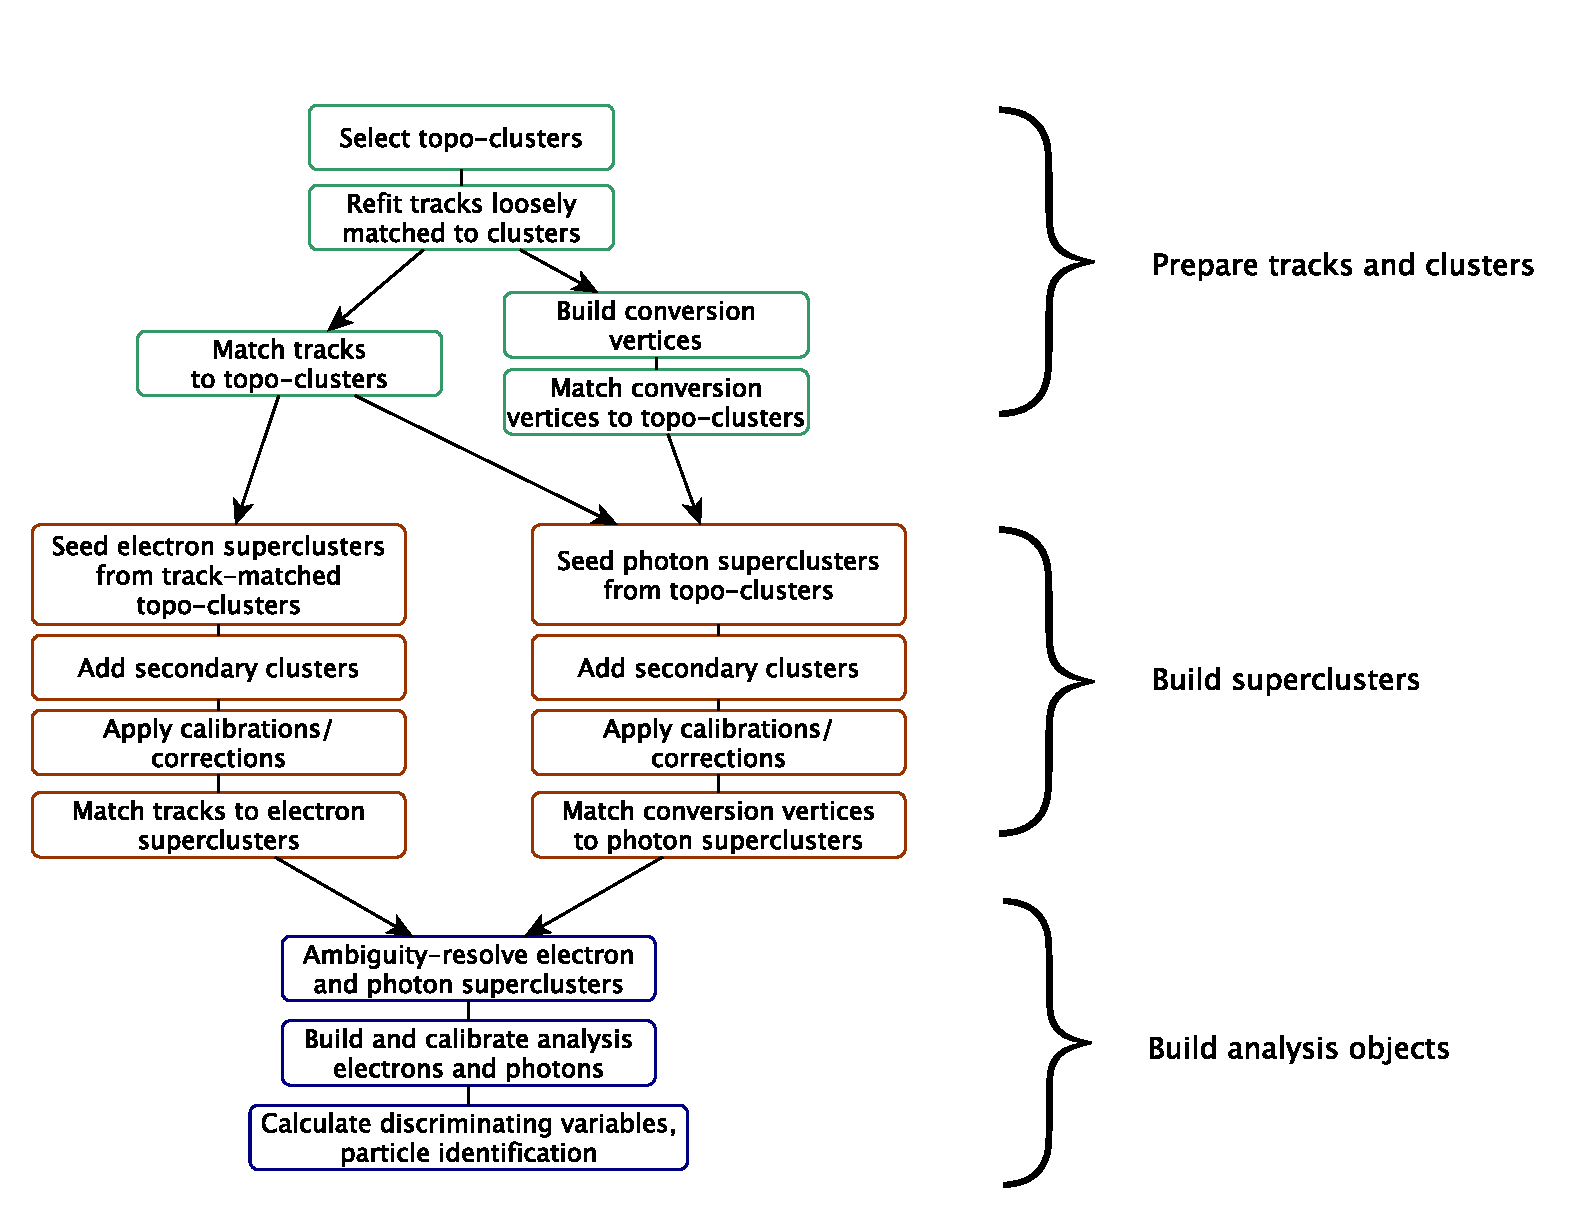
\includegraphics[width=0.8\linewidth]{3_experiment/object_reconstruction/egamma_reconstruction}
    \caption{Diagrama del algoritmo de reconstrucción de electrones and fotones, extraído de \Refn{\cite{ATLAS-EGamma-Performance-2015-2017}}}
    \label{fig:objects:egamma:reco:reco_diagram}
\end{figure}

El algoritmo para la reconstrucción de electrones y fotones procede como se muestra en la \Fig{\ref{fig:objects:egamma:reco:reco_diagram}}.
El proceso de reconstrucción comienza con la formación de \topos. Primero se forman proto-clusters en el \ac{ECAL} y \ac{HCAL} agrupando celdas que tienen una energía requerida y predefinida y añadiendo posteriormente celdas vecinas obteniendo así los \topos. Las reconstrucciones continúan sólo en aquellos casos en los que la energía de los \topos en el \ac{ECAL} es superior a \(400~\mev\) y la fracción de la misma con respecto a la energía total del \topo es mayor a \(0.5\), reduciendo gran parte los efectos de pileup.

El algoritmo también construye vértices de conversión a partir de las trazas reajustadas y los empareja con los \topos seleccionados.
Tras el ajuste inicial de las trazas y la construcción de las conversiones, los algoritmos de superclusters de electrones y fotones se ejecutan por separado y en paralelo. En la primera etapa, los \topos se evalúan para su uso como candidatos a clusters semilla que forman la base de los superclusters; en la segunda etapa, los clusters cercanos a los candidatos a clusters semilla se identifican como candidatos a clusters satélite que pueden surgir de la radiación bremsstrahlung o de la división de los \topos. Los clusters satélite que superan ciertos criterios de selección, se añaden a los candidatos a semilla para formar los superclusters finales.
Finalmente el algoritmo de reconstrucción hace coincidir las trazas con los superclusters de electrones y los vértices de conversión a los superclusters de fotones.

Dado que un objeto puede reconstruirse como electrón y como fotón, se resuelve esta ambigüedad para eliminar parte del solapamiento. Sin embargo, se permite cierto solapamiento para mantener una alta eficiencia de reconstrucción de electrones y fotones y para que en cada análisis de datos se apliquen criterios específicos a dicho estudio. Finalmente, se construyen y calibran los objetos finales.



\subsection{Identificación}
\label{subsec:objects:egamma:id}

Con el objetivo de poder discriminar los objetos \textit{prompt}\footnote{El término \textit{prompt} hace referencia a aquellos objetos producidos rápidamente luego de la colisión, generalmente provenientes del vértice primario, para distinguirlos de aquellos producidos por el decaimiento tardío de otra partícula, como puede ser un hadrón.} de aquellos que no lo son, existen diferentes criterios de identificación.
En \ac{ATLAS}, la identificación de fotones y electrones se logra mediante una serie de variables denominadas \acfp{SS} (descriptas en detalle en \Ch{\ref{ch:pid_ss}}). Estas son variables que describen el paso de los fotones y electrones a través del \ac{ECAL} y \ac{HCAL}, caracterizando las lluvias electromagnéticas en su desarrollo lateral y longitudinal y son calculadas a partir de la energía depositada en las celdas de estos calorímetros. Mediante ciertos algoritmos que hacen uso de las \acp{SS}, se logra incrementar la pureza de los objetos deseados al costo de tener una menor eficiencia de selección.
Finalmente, se definen diferentes \acp{WP} que son derivados de forma central y luego distribuidos a toda la colaboración.

El objetivo principal de la identificación de electrones es separar los electrones prompt de los electrones producto del proceso de creación de pares a partir de los fotones, de los jets que depositan energía en el \ac{ECAL} y de los electrones provenientes del decaimiento de hadrones originados por quarks de sabores pesados (\textit{heavy-flavor}). La identificación se basa en un método likelihood que utiliza algunas de las \acp{SS}, utilizando electrones provenientes de decaimientos de \jpsi y \Zboson para bajo y alto \et, respectivamente~\cite{ATLAS-EGamma-Performance-2024}. Se definen entonces \acp{WP}, denominados \texttt{Loose}, \texttt{Medium} y \texttt{Tight}, cuyas eficiencias de identificación de un electrón con \(\et=40~\gev\) son de \(93\%, \, 88\%\) y \(80\%\), respectivamente~\cite{ATLAS-EGamma-Calibration-2015-2016}.


Para distinguir los fotones prompt/reales (los procedentes de la colisión) de los fotones de fondo (procedentes del decaimiento de hadrones, también llamados fotones falsos), es necesario basarse en un algoritmo de identificación con alta eficiencia de señal y rechazo de fondo para fotones candidatos con \(\pt \sim 10~\gev\) hasta la escala \tev.
Actualmente, la identificación de fotones en \ac{ATLAS} se basa en un conjunto de cortes rectangulares en las \acp{SS} mencionadas anteriormente.
El proceso completo de identificación de fotones se presenta en \Ch{\ref{ch:pid_ss}}, donde las \acp{SS} se explican una a una. Además, en el \Ch{\ref{ch:ss_corrections}} se presentan dos enfoques para corregir las diferencias observadas en estas variables entre los datos y \ac{MC}, uno de los objetivos de esta tesis.





\subsection{Aislamiento}
\label{subsec:objects:egamma:iso}

Para mejorar aún más la selección de fotones y electrones se aplican criterios de aislamiento a estos objetos. Para ello, se definen dos criterios de aislamiento: calorimétrico y de trazas. 

\begin{figure}[ht!]
    \centering
    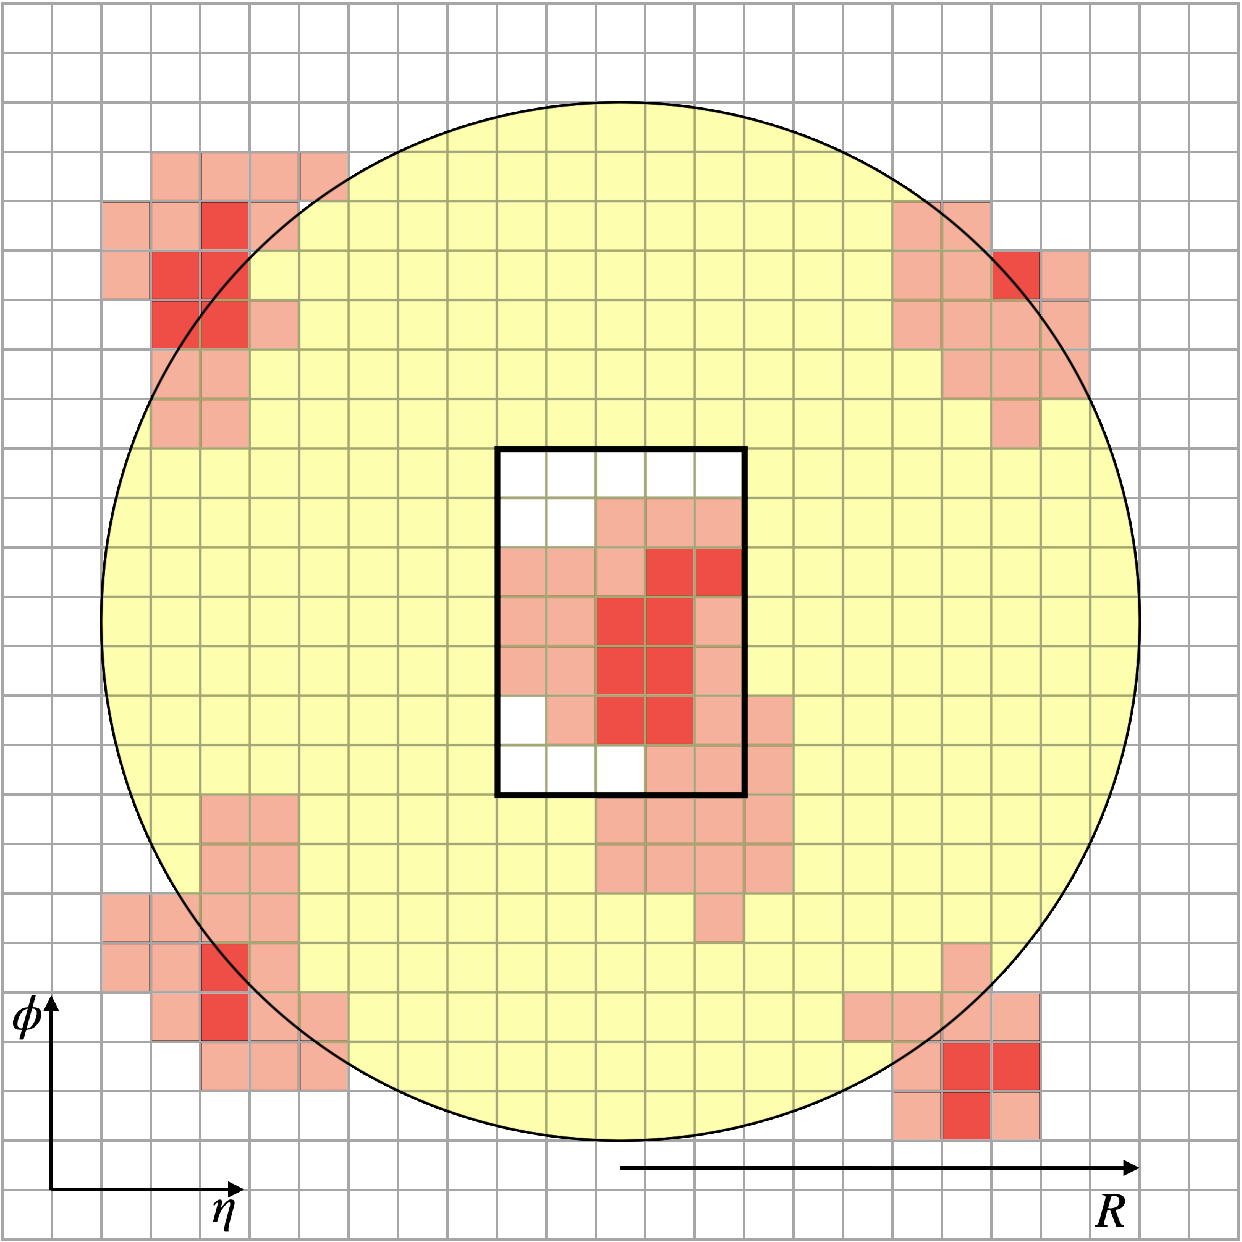
\includegraphics[width=0.5\linewidth]{3_experiment/object_reconstruction/isolation_diagram}
    \caption{Diagrama del proceso del cálculo de la variable de aislamiento calorimétrico. Cuando se utiliza un cono con \(R=0.4\), se puede construir la variable \etconefo mencionada en el texto.}
    \label{fig:objects:egamma:iso:iso_diagram}
\end{figure}

El procedimiento para calcular la energía de aislamiento calorimétrico \etconefo se esquematiza en la \Fig{\ref{fig:objects:egamma:iso:iso_diagram}}. En primer lugar se construye un cono de radio \(\DeltaR<0.4\) alrededor del candidato a fotón o electrón y se suman las energías de todas las celdas de los \topos (introducidos en la \Sect{\ref{subsec:objects:egamma:reco}}) cuyos baricentros se encuentran dentro del cono. A continuación, a esta energía calculada se le resta la energía de todas las celdas en una ventana de \(5\times 7\) (en unidades de \(\eta \times \phi\) en la segunda capa del \ac{ECAL}) centrada alrededor del candidato, con el fin de eliminar la energía del propio candidato.
También se realizan correcciones para tener en cuenta las fugas de energía fuera del cono y las contribuciones de pileup~\cite{PileupSubstraction}. La forma final de la energía de aislamiento calorimétrico resulta:
\begin{equation*}
    \etconefo  = E_{T,\text{raw}}^{\text{isol}40} - E_{T,\text{core}} - E_{T,\text{leakage}} - E_{T,\text{pileup}}
\end{equation*}


La variable de aislamiento de trazas, \ptconetw se obtiene sumando los \pt de las trazas de buena calidad en un cono de radio \(\DeltaR<0.2\) alrededor del candidato a electrón o en la dirección del cluster de fotones convertidos.
Se excluyen de este cómputo las trazas asociadas a la traza o al fotón convertido así como aquellas trazas que no pasan el requisito de trazas de buena calidad. Una traza de buena calidad se define como aquella en la que el \(\pt>1~\gev\) y tiene una distancia mínima al vértice primario a lo largo del eje \(z\) de \(|z_0 \sin \theta| < 3\) mm.

En general, para los fotones y electrones no hay otra energía depositada en el cono alrededor del candidato, aparte de los objetos de baja energía originados por los restos de la colisión, las interacciones múltiples y el pileup. En cambio, para los falsos candidatos a fotones y los fotones no directos se observa energía adicional dentro del cono proveniente de los objetos que los acompañan en el jet.

\begin{table}[ht!]
    \caption{Resumen de los \ac{WP} de aislamiento para electrones y fotones usados a lo largo de esta tesis.}
    \resizebox{\linewidth}{!}{
        \begin{tabular}{|l|c|c|c|}
            \hline
            Objecto                      & \ac{WP}                             & Aislamiento Calorimétrico                                    & Aislamiento de trazas   \\ \hline
            \multirow{3}{*}{Fotón}     & \texttt{Loose}         & \(E_{T}^{\text{cone20}}<0.065\times \pt \)                & -                                  \\
                                        & \texttt{TightCaloOnly} & \(\etconefo < 0.022\times \pt + 2.45~\gev\)               & -                                  \\
                                        & \texttt{Tight}         & \(\etconefo < 0.022\times \pt + 2.45~\gev\)               & \(\ptconetw/\pt < 0.05\)           \\ \hline
            Electrón   & \texttt{Loose\_VarRad}         & \(\etconetw < 0.2\times\pt\)                              & \(\pt^{\text{cone30}}/\pt < 0.15\) \\
                                        % & \texttt{HighPtCaloOnly}        & \(\etconetw < \max\left(0.015\times\pt, 3.5~\gev\right)\) & -                                  \\ 
            \hline
        \end{tabular}
    }
    \label{fig:objects:egamma:iso:iso_table}
\end{table}

A partir del aislamiento calorimétrico y de trazas se pueden definir diferentes \acp{WP} por separado tanto para electrones como para fotones. En el caso de los electrones se definen dos estrategias: o bien conseguir una eficiencia fija, o aplicar cortes fijos en las variables de aislamiento. En el caso de los fotones, hay \acp{WP} que no utilizan ambas variables de aislamiento, como es el caso del \ac{WP} que sólo utiliza el aislamiento calorimétrico. Las definiciones de los diferentes \acp{WP} utilizados a lo largo de esta tesis se muestran en la \Tab{\ref{fig:objects:egamma:iso:iso_table}}. Además, es común definir las siguientes variables para el \ac{WP} \texttt{FixedCutTight} del fotón:
\begin{align}
    \label{eq:objects:egamma:iso:definitions}
    \etiso &= \etconefo - 0.022 \times \et - 2.45~\gev\\
    \ptiso &= \ptconetw / \et
\end{align}
lo que resulta para el \ac{WP} \texttt{FixedCutTight} en:
\begin{align}
    \etiso &< 0 ~\gev\\
    \ptiso &< 0.05.
\end{align}















\section{Muones}



La tasa de radiación bremsstrahlung es inversamente proporcional al cuadrado de la masa de una partícula. Dado que los muones son unas 200 veces más pesados que los electrones, interactúan principalmente con el material del detector a través de ionización. Por lo tanto, los muones son partículas mínimamente ionizantes que no crean lluvia electromagnética en los calorímetros y atraviesan todas las capas del detector \ac{ATLAS}. Es por esta razón que la detección de muones depende de las mediciones de las trazas dejadas por ellos en el \ac{ID} y el \ac{MS}. La combinación de los dos subdetectores define cuatro tipos de muones, dependiendo de la información utilizada para la reconstrucción:
\begin{itemize}
    \item \ac{CB}: muón reconstruido a partir de un reajuste global de las trazas del \ac{ID} y del \ac{MS},
    \item \ac{ST}: muón reconstruido a partir de una traza ajustada del \ac{ID} que al extrapolarla al \ac{MS} tienen un segmento en el \ac{MDT} o el \ac{CSC},
    \item \ac{CT}: muón reconstruidos a partir de la traza del \ac{ID} ajustada a los depósitos de mínima energía ionizante en los calorímetros,
    \item \ac{ME}: muón reconstruido únicamente a partir de las trazas \ac{MS}.
\end{itemize}

El solapamiento entre distintos tipos de muones se resuelve del siguiente modo. Cuando dos tipos de muones comparten la misma traza del \ac{ID}, el orden de preferencia es: primero el \ac{CB}, luego el \ac{ST} y finalmente el \ac{CT}. El solapamiento con \ac{ME} se resuelve analizando los hits de las trazas seleccionando aquellas trazas con mejor ajuste y mayor número de hits.

Para la identificación de muones se aplican cortes de calidad para distinguir los muones aislados de los procedentes de procesos de fondo, principalmente del decaimiento de piones y kaones.
Las variables con buen poder discriminatorio utilizadas se describen en \Refn{\cite{ATLAS-Muon-Performance-2016}}. Se definen cuatro selecciones de identificación: \texttt{Loose}, \texttt{Medium}, \texttt{Tight} y \texttt{High-pT}. Las tres primeras categorías son inclusivas, siendo \texttt{Medium} la selección por defecto en \ac{ATLAS}. Por último, se pide a los candidatos a muones que van a ser utilizados por los análisis que satisfagan los requisitos de aislamiento, tanto a nivel de trazas como calorimétricos, de forma análoga a los detallados para los electrones y fotones en el apartado anterior. Para el aislamiento de trazas, se utiliza una variable similar a la empleada para los electrones fotones pero con un cono de radio variable \(\DeltaR = \min(10~\gev/\pt, 0.3)\) alrededor del momento del muón excluyendo la traza del mismo. Para el aislamiento calorimétrico se utiliza la misma variable \etconefo con la diferencia de utilizar un radio de \(R=0.2\) en lugar de \(0.4\). En base a estas variables, se definen 7 criterios de selección de aislamiento (7 \acp{WP}), optimizados para diferentes análisis.








\section{Jets}
\label{sec:objects:jets}

Los quarks y gluones no pueden detectarse de manera aislada, sino que por un proceso denominado hadronización dan lugar a un chorro colimado de partículas que se denomina \textit{jet}. Estos penetran a través del \ac{ECAL} y son totalmente absorbidos por el material del calorímetro hadrónico. A continuación, se describen los métodos de reconstrucción de jets utilizados en \ac{ATLAS}

\subsection{Algoritmo de clusterización de jets \texorpdfstring{\antikt}{Anti-kT}}

Dado que los jets están constituidos por un elevado número de partículas que dejan deposiciones de energía en el \ac{ECAL} y \ac{HCAL} y trazas en el \ac{ID}, un algoritmo de clusterización agrupa los constituyentes en el evento para definir los jets. Dicho algoritmo se denomina algoritmo \antikt~\cite{AntiKtAlgorithm}. Del mismo modo que para los electrones y los fotones, la reconstrucción de los jets en \ac{ATLAS} comienza en la formación de \topos: depósitos de energía agrupados en las celdas de los calorímetros mediante un algoritmo de combinación secuencial. Entonces, el algoritmo \antikt combina los \topos con los siguientes pasos:
\begin{itemize}
    \item Determinación de la distancia entre todos los \topos entre sí y de cada \topo con el haz:
        \begin{gather}
            \dij = \min \left( p_{T,i}^{-2}, p_{T,j}^{-2} \right) \frac{\Delta_{i,j}^2}{R^2}\\
            d_{iB} = p_{T,i}^{-2}
        \end{gather}
        donde \(\Delta_{ij}^2 = \Delta\phi_{ij}^2 + \Delta\eta_{ij}^2\) y \(R\) es un valor fijo del algoritmo que define el radio jet.
    \item Si el mínimo de todas las distancias calculadas anteriormente es \(d_{iB}\), el \topo \(i\) se clasifica como jet y se descarta en iteraciones sucesivas.
    \item Si \(d_{ij} < d_{iB}\) se combinan los \topos \(i\) y \(j\), todas las distancias se calculan nuevamente con este nuevo \topo y la iteración se realiza de nuevo.
\end{itemize}
Este proceso se repite hasta que todas las partículas del evento se han agrupado.

El algoritmo \antikt tiende a unificar las partículas \textit{soft} con las \textit{hard} y a separar a las partículas \textit{hard} entre sí, ya que la partícula con mayor \pt definirá el término \(\min \left( \frac{1}{p_{T,i}^2}, \frac{1}{p_{T,j}^2}  \right)\) en la definición de \dij. Esto permite que los jets del evento tengan una dirección estable al principio del proceso de combinación. El algoritmo \antikt es preferible a otros algoritmos secuenciales de jets ya que los jets tienen formas regulares que son aproximadamente cónicas, mostrados en la \Fig{\ref{fig:objects:jets:antikt}}. Los jets que se originan a partir de quarks o gluones en general se denominan small-\(R\) jets y para su reconstrucción se utiliza un radio de \(R=0.4\). Por otro lado, los jets que representan partículas masivas que decaen hadrónicamente se denominan large-\(R\) jets y se utiliza \(R=1.0\), dado que el uso de un cono más amplio ayuda a incluir la mayoría de las partículas producto del decaimiento.


\begin{figure}[ht!]
    \centering
    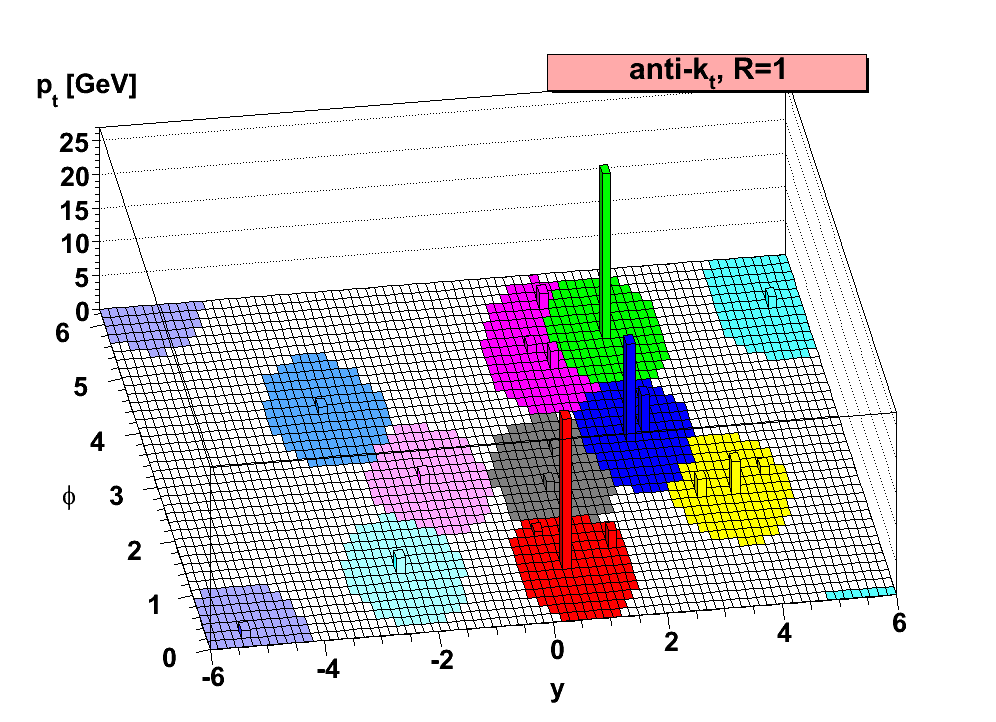
\includegraphics[width=0.7\linewidth]{3_experiment/object_reconstruction/antikt_clusters}
    \caption{Representación esquemática del algoritmo \antikt para el proceso de clusterización de jets~\cite{AntiKtAlgorithm}.}
    \label{fig:objects:jets:antikt}
\end{figure}

\subsection{Jets Calorimétricos}

Una forma de reconstruir los jets se basa en los depósitos de energía en el calorímetro. De forma similar a lo que se ha explicado para electrones y fotones en la \Sect{\ref{subsec:objects:egamma:reco}}, los depósitos de energía en las celdas del \ac{ECAL} y \ac{HCAL} se utilizan para construir \topos, cuyas energías se aproximan a las depositadas por los hadrones individuales~\cite{ATLAS-TopoClusters-Run1,ATLAS-TopoClusters-Run2}. Los jets reconstruidos de esta manera y agrupados con el algoritmo \antikt con un radio de \(R=0.4\) se denominan jets \textsc{EMTopo}. En la reconstrucción de jets, sólo se incluyen los \topos con energía neta positiva.

\subsection{\acf{PFlow} Jets}

Otro método para la reconstrucción de jets se basa en el algoritmo \ac{PFlow}~\cite{ATLAS-JetPFlow-Performance}, en el que las mediciones del \ac{ID} y del calorímetro se combinan para formar las señales que idealmente representan partículas individuales. El algoritmo comienza vinculando cada traza del \ac{ID} con un solo \topo y calcula la energía esperada en el calorímetro depositada por cada partícula que también inició la traza. Luego, para cada sistema \topo/traza, el algoritmo evalúa la probabilidad de que la energía de la partícula haya sido depositada en más de un \topo y decide si es necesario agregar más \topos al sistema \topo/traza para recuperar la energía total del la lluvia. Posteriormente, la energía depositada por la partícula que inicia la traza es sustraída celda por celda del conjunto de \topos vinculados. Finalmente, si la energía remanente en el sistema es consistente con la esperada por las fluctuaciones de la lluvia de la señal de una sola partícula, los remanentes del \topo son removidos.

El resultado de este algoritmo es un conjunto de trazas, el conjunto de \topos y otro conjunto de \topos modificados por el procedimiento anterior. La combinación de estos 3 conjuntos definen un objecto \ac{PFlow}. Estos objetos también pueden ser agrupados con el algoritmo \antikt y con \(R=0.4\) para formar los jets \ac{PFlow}.

El algoritmo \ac{PFlow} tiene bastantes ventajas sobre el \textsc{EMTopo}:
\begin{itemize}
    \item La resolución en \pt del \ac{ID} es significativamente mejor que la resolución de energía del calorímetro para partículas cargadas de baja energía.
    \item Permite una mayor aceptancia para partículas más \textit{soft}. Las trazas se reconstruyen para partículas cargadas con un mínimo \pt de \(400~\mev\), el cual es menor que el requerido para la formación de \topos.
    \item Mejora la resolución angular de una sola partícula cargada ya que utiliza la información del \ac{ID} en lugar de la del calorímetro.
    \item Las partículas cargadas de bajo \pt que se originan dentro de un jet hadrónico son barridas fuera del cono del jet por el campo magnético para cuando alcanzan el calorímetro. Utilizando la coordenada azimutal de las trazas en el perigeo, estas partículas también son agrupadas en el jet.
    \item Es posible eliminar las trazas originadas por el pileup, sabiendo que éstas no proceden del \ac{PV}.
\end{itemize}

Cabe mencionarse, sin embargo, que para cualquier partícula cuya traza deba utilizarse, es necesario identificar correctamente y sustraer su señal en el calorímetro para evitar un doble conteo. En el algoritmo \ac{PFlow} se toma una decisión booleana sobre si utilizar la medición del \ac{ID} o del calorímetro. La capacidad de sustraer con precisión toda la energía de una sola partícula, sin eliminar la energía depositada por otras partículas, constituye el criterio clave de rendimiento sobre el que se optimiza el algoritmo.

En esta tesis, se consideran los jets \ac{PFlow} ya que han demostrado proporcionar una mejor reconstrucción del jet~\cite{ATLAS-JetPFlow-Performance}.


\subsection{Calibración de jets}

Una vez reconstruidos los jets, su cuadrimomento se corrige para que coincida con la cinemática de un \textit{truth}-jet\footnote{Los truth jets, o jets reales, son jets asociados a una partícula específica (jet iniciado por un quark de sabor liviano, por ejemplo) proveniente del estado final de una simulación luego de pasar por el algoritmo de clusterización \antikt.}. Las tres primeras correcciones tienen en cuenta la contaminación de la distribución de pileup subyacente y las fluctuaciones debidas al origen del jet~\cite{ATLAS-Jet-Calibration-Run2}. La \textit{Global Sequential Calibration} mejora la resolución de \pt de los jets (y las incertidumbres asociadas) eliminando secuencialmente la dependencia de la respuesta reconstruida del jet (\(R= E^{\text{reco}} / E^{\text{truth}}\)) en diversos observables. Por último, las diferencias residuales entre los datos y \ac{MC} se tienen en cuenta midiendo el desequilibrio de momento en \Zjets, \gammajet y eventos multijet.

Para reducir el número de jets con una fracción considerable de energía procedente del pileup, se utiliza un algoritmo basado en redes neuronales denominado \ac{NNJvt} (sucesor de \ac{JVT}~\cite{ATLAS-JetPileup-Run1}). Este algoritmo reconstruye un discriminante multivariable que combina, entre otras cantidades, el \ac{JVF} (fracción de las trazas \pt asociada a un jet originado por el \ac{PV} y el número total de trazas) y el número de \acp{PV} en el evento \Npv. Como los jets que no proceden de la interacción fuerte son generalmente de más baja energía, el corte \ac{JVT} se aplica sólo a los jets con \(\pt<60~\gev\) y \(\abseta<2.4\). El \ac{WP} por defecto del \ac{NNJvt} tiene una eficiencia en el rango de \(88-99\%\) para los jets con \(20<\pt<60~\gev\).


















\section{Jets provenientes de quarks pesados (Jets \textit{heavy flavor})}
\label{sec:objects:ftag}

Los decaimientos de hadrones pesados (de ahora en más heavy-flavor) se rigen principalmente por el hadrón más pesado en la cascada de decaimiento. Un hadrón \(b\) generalmente decae en cascada a un hadrón \(c\), que a su vez decae a un hadrón \(s\), etc., lo que conduce a la existencia de múltiples vértices.

\ac{FTAG} es la clasificación de los jets dependiendo del sabor (\textit{flavor}) de los quarks por los que fueron iniciados, utilizando algoritmos sensibles a las propiedades distintivas de las respectivas clases. Entre ellos se consideran jets iniciados quarks \(b\) (\bjets), \(c\) (\cjets) o ni \(b\) ni \(c\) (jets livianos, también referidos como light-jets o \ljets).
Estos complejos algoritmos se basan en los múltiples vértices, en la elevada masa, la alta multiplicidad de decaimientos y los modos de decaimiento característicos de los hadrones \(b\) y \(c\), así como en las propiedades de la fragmentación de los quarks pesados.


En \ac{ATLAS} se emplea un proceso de dos etapas para reconstruir las características más relevantes de los jets heavy-flavor. En la primera etapa, los algoritmos de bajo nivel utilizan métodos complementarios para extraer información sobre las trazas de las partículas cargadas vinculadas al jet. Algunos algoritmos se centran en las propiedades de las trazas individuales, mientras que otros analizan sus correlaciones o las combinan para reconstruir explícitamente los vértices desplazados. En la segunda etapa, las salidas de estos algoritmos se integran en un algoritmo de alto nivel que utiliza clasificadores multivariables para optimizar el rendimiento. Con el tiempo, los algoritmos han evolucionado significativamente, empezando con discriminantes basados en likelihoods y \acp{BDT} durante el Run-1 del \ac{LHC}, y avanzando hacia métodos más avanzados como las redes neuronales recurrentes y profundas, lo que ha dado lugar a notables mejoras en el rendimiento de la identificación~\cite{ATLAS-FTAG-Calibration-2012,ATLAS-FTAG-Efficiency-2012,MV2Algorithm,ATLAS-FTAG-DeepLearning}.

A partir del Run-3, el grupo de \ac{ATLAS} \ac{FTAG}, desarrolla un novedoso algoritmo \enquote{GN2} basado en un transformador~\cite{GN2Transformer}. El algoritmo GN2 es un único modelo entrenado que sustituye a DL1d~\cite{ATLAS-FTAG-DL1-Run2} y a los algoritmos de bajo nivel que lo alimentan. Se basa en GN1~\cite{ATLAS-FTAG-GN1}, que se refinó para pasar a ser GN2. GN2 sustituye la \textit{Graph Attention Network}~\cite{GANs} utilizada por GN1 por un Transformador, y también se beneficia de otras optimizaciones de arquitectura y la posibilidad de entrenamiento de la red con un orden de magnitud más de datos.

El algoritmo toma directamente información sobre el jet y las trazas asociadas y, como tal, no depende de otros algoritmos de etiquetado de sabores (\textit{flavor tagging}). Mantiene los dos objetivos de entrenamiento auxiliares que se introdujeron con GN1: la agrupación de trazas que se originan en un vértice común y la predicción del proceso físico subyacente del que se originó cada traza.

Este nuevo algoritmo también está preparado para proporcionar la identificación de \cjets y jets procedentes de decaimientos \(\tau\). Las salidas de este tagger corresponden a las probabilidades de que un jet sea etiquetado (\textit{taggeado}) como un jet \(b\), \(c\), \(\tau\) o \textit{light}, denominadas como \(p_b\), \(p_c\), \(p_{\tau}\) y \(p_u\), respectivamente.

\subsection{Identificación y performance de \btagging}

Para evaluar la capacidad del tagger de identificar \bjets con una eficiencia constante, se mide la capacidad de rechazar los jets \(c\), \(\tau\) y light. Las probabilidades de salida del tagger se combinan para construir un único discriminante \gntb, definido como
\begin{equation}
    \gntb = \log \left(
        \frac{p_b}{f_c p_c + f_{\tau} p_{\tau} + \left(1-f_c-f_{\tau}\right)p_u}
    \right).
\end{equation}
Los parámetros \(f_{c(\tau)}\) son libres y determinan la importancia entre \(p_{c(\tau)}\) y \(p_u\) en el discriminante. Los valores específicos de estos parámetros se determinan mediante un procedimiento de optimización maximizando el rechazo de \cjets (\(\tau\)-jets) y \ljets y resultan ser \(0.2\) (\(0.01\)).


A partir del valor discriminante del tagger, se pueden definir varios \acp{WP} exigiendo que el valor \gntb esté por encima de un determinado umbral. El grupo \ac{FTAG} de \ac{ATLAS} proporciona de forma centralizada a toda la colaboración cinco \acp{WP} diferentes para lograr una eficiencia global fija de \btagging: \(65,\, 70,\, 77,\, 85\) y \(90\%\), que se muestran en la \Fig{\ref{fig:objects:jet_tagging:btag_discrminant}}. En dicha figura se comparan también las distribuciones de datos y \ac{MC} del tagger GN2, donde las contribuciones de los distintos sabores se muestran con colores diferentes.

\begin{figure}[ht!]
    \centering
    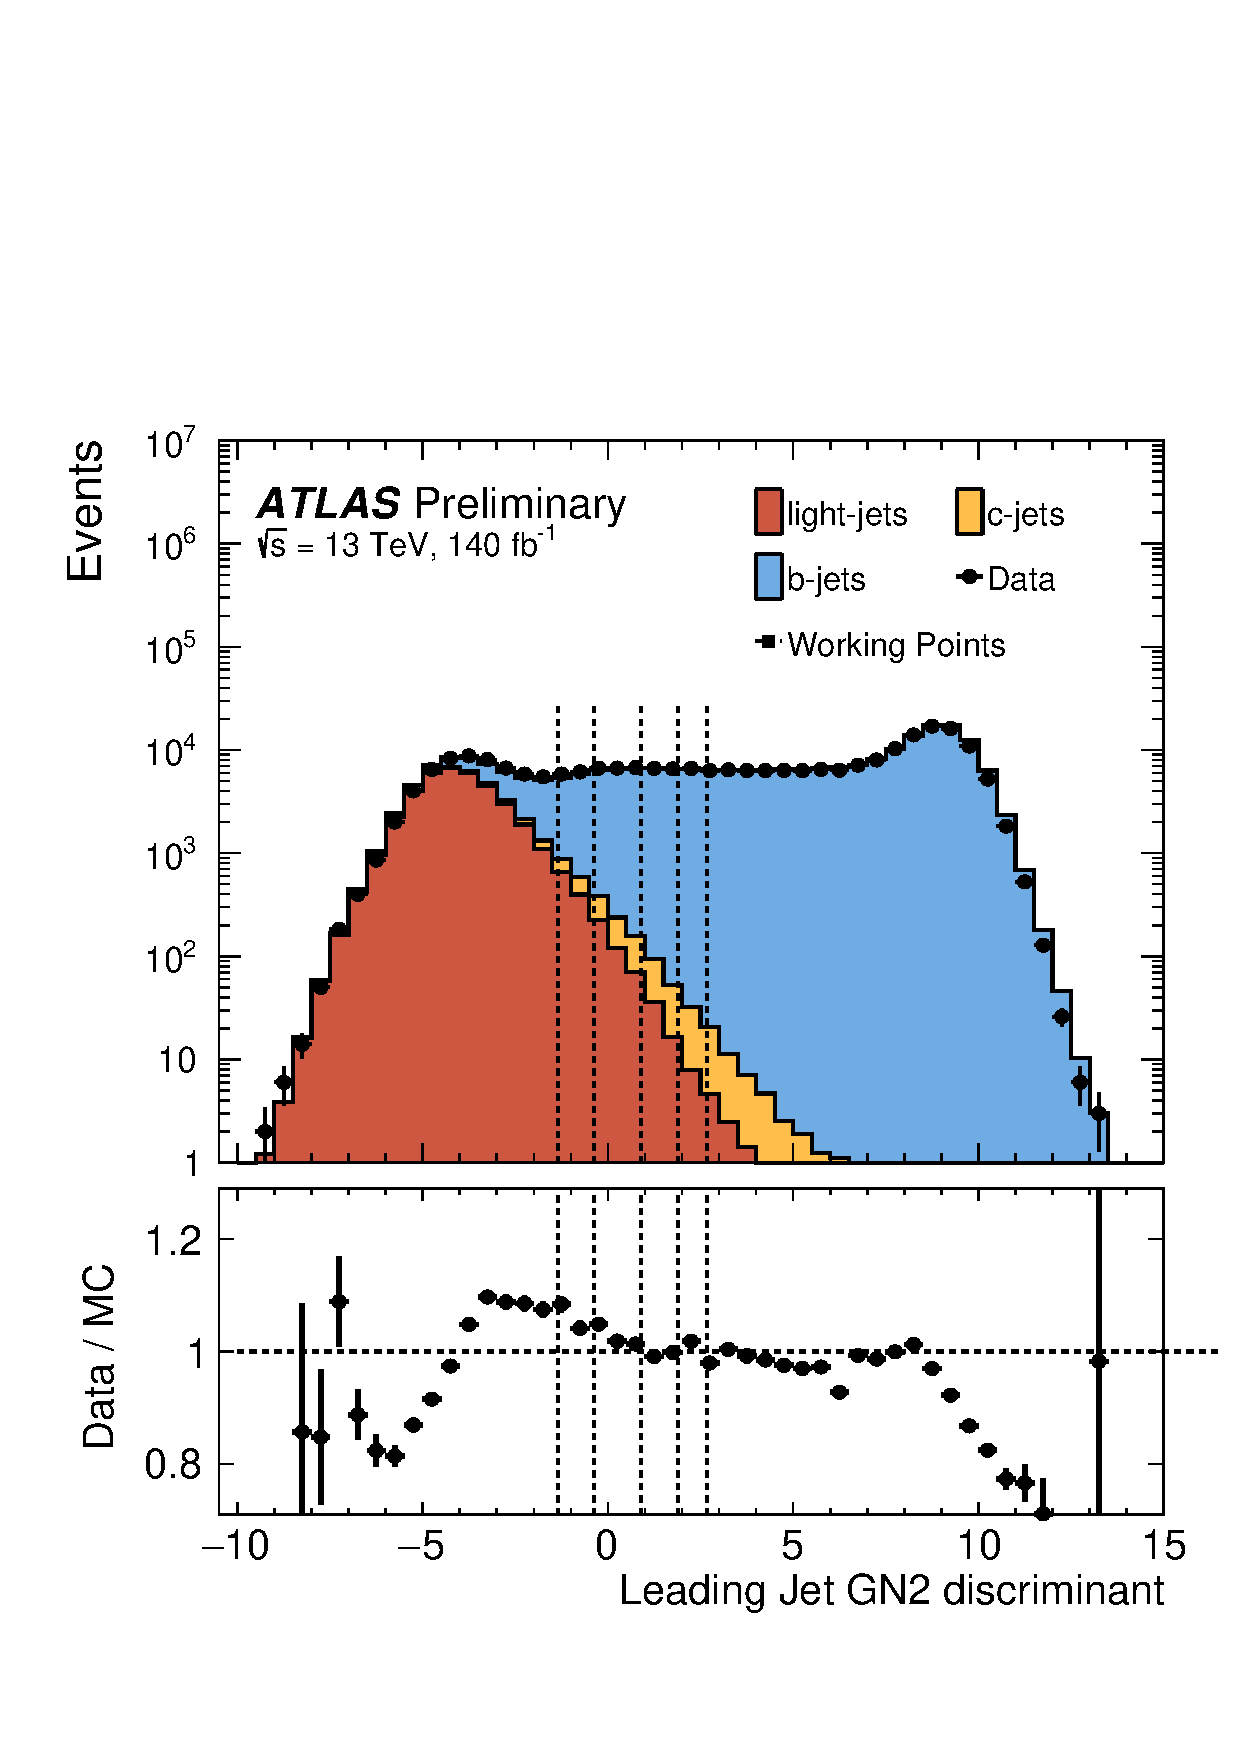
\includegraphics[width=0.6\linewidth]{3_experiment/object_reconstruction/btagging_discriminant}
    \caption{Comparación entre datos y simulación \ac{MC} (eventos del proceso \ttbar semileptónico) del discriminante del tagger GN2. Las contribuciones de los jets \(l\), \(b\) y \(c\) se muestran con diferentes colores, y los 5 \acp{WP} de \btagging se muestran con las líneas verticales punteadas. De izquierda a derecha, las líneas representan los \acp{WP} de \(90, 85, 77, 70\) y \(65\%\) de eficiencia. El panel inferior muestra el ratio entre los datos y la suma de las simulaciones \ac{MC}~\cite{ATLAS-FTAG-GN2BtagWPs}.}
    \label{fig:objects:jet_tagging:btag_discrminant}
\end{figure}

Uno de los principales problemas del \btagging es la disminución de la eficiencia a mayor \pt. En este régimen de \pt elevado las partículas están más colimadas y tienden a viajar más lejos en el \ac{ID} antes de decaer, lo que puede dar lugar a una traza de decaimiento con hits espurios. La degradación de la eficiencia se visualiza en la \Tab{\ref{tab:objects:ftag:btag_efficiency_original}}, donde se muestran las eficiencias de tagging para \bjets, junto con los rechazos a \cjets, \ljets y \tjets, en los regímenes de bajo y alto \pt. Los valores mostrados se calculan utilizando diferentes muestras en las que \ttbar se utiliza en la región de bajo \pt y eventos de decaimiento de \(Z'\)~\footnote{El modelo leptofóbico de vector axial \(Z'\) es un modelo de Materia Oscura simplificado en el cual el decaimiento teorizado es un par de quarks.} se utilizan en la región de alto \pt. Puede verse que la eficiencia de \btag cae en un \(30\%\) para jets de \pt más alto.

\begin{table}[ht!]
    \caption{Medidas de eficiencias de \btagging, y de rechazos de \cjets, \ljets y \tjets, en los regímenes de bajo y alto \pt.}
    \label{tab:objects:ftag:btag_efficiency_original}
    \resizebox{\textwidth}{!}{
        \begin{tabular}{llcccc}
            \toprule
            Muestra & Rango de \pt [\gev]   & Eficiencia de \bjet & Rechazo de \cjet & Rechazo de \ljet & Rechazo de \tjet \\ \midrule
            $t\bar{t}$  & \(20<\pt<250\)    & $0.76$              & $17.52$          & $448.61$         & $71.15$          \\
            $Z'$        & \(250<\pt<6000\)  & $0.41$              & $20.27$          & $179.99$         & $452.94$         \\ \bottomrule
        \end{tabular}
    }
\end{table}

\subsection{Identificación y performance de \ctagging}

Al igual que con \btagging, se puede construir un único discriminante a partir de las probabilidades dadas por el tagger para identificar \cjets frente a \bjets, \tjets y \ljets:
\begin{equation}
    \gntc = \log \left(
        \frac{p_c}{f_b p_b + f_{\tau} p_{\tau} + \left(1-f_b-f_{\tau}\right)p_u}
    \right)
\end{equation}
donde ahora los valores \(f_{b(\tau)}\) son los parámetros libres que controlan el rechazo entre jets \(b\), \(\tau\) y light. Utilizando el mismo procedimiento de optimización que para \btagging, los valores para \(f_{b(\tau)}\) resultan ser \(0.3\) (\(0.05\)).

Gracias a la gran eficiencia de \btagging conseguida por GN2, es posible diseñar un \ac{WP} de \ctagging tras aplicar un veto de \btagging separando aún más los \cjets de los \ljets. Construyendo este \ac{WP} de tagging simultáneo y suponiendo que la fracción de \tjets es despreciable se pueden separar los jets \(b\), \(c\) y livianos en tres regiones ortogonales. Partiendo de exigir que un jet \textit{no} pase el \ac{WP} de \btagging de \(77\%\) de eficiencia (veto \btag), se definen tres \acp{WP} diferentes de \ctagging definidos para eficiencias de \(10, \, 30\) y \(50\%\) fijando el valor de \gntc. Las medidas de eficiencia y rechazo de las dos muestras descriptas anteriormente tras aplicar el \ac{WP} de \ctag de \(50\%\) de eficiencia se muestran en el \Tab{\ref{tab:objects:ftag:ctag_efficiency_original}}.

\begin{table}[ht!]
    \caption{Medidas de eficiencia de \ctagging para \cjets, y valores de rechazos de \bjets, \ljets y \tjets en los regímenes de bajo y alto \pt. Los valores corresponden a aquellos luego de aplicar el veto del \ac{WP} de \btagging de \(77\%\) y de \(50\%\) de \ctagging}
    \label{tab:objects:ftag:ctag_efficiency_original}
    \resizebox{\linewidth}{!}{
        \begin{tabular}{llcccc}
            \toprule
            Muestra & Rango de \pt [\gev]   & Eficiencia de \cjet & Rechazo de \bjet & Rechazo de \ljet & Rechazo de \tjet \\ \midrule
            $t\bar{t}$  & \(20<\pt<250\)    & $0.467$             & $8.11$           & $26.77$          & $9.52$           \\
            $Z'$        & \(250<\pt<6000\)  & $0.344$             & $5.34$           & $13.09$          & $275.22$         \\ \bottomrule
        \end{tabular}
    }
\end{table}